% $  Id: validation.tex  $
% !TEX root = main.tex


%%
\section{Validation}
\label{sec:validation}

\authorcomment[missing]{}{Glue text to the section}


%%%%
\subsection{Environment of execution}
Because the first project data and guidance was provided by Google's Machine Learning Crash course~\cite{mlchrome18}  it was run directly on the Google Chrome browser using their Colaboratory platform. Nonetheless, it is possible to execute the program offline which requires the user to set up a local Datalab environment by installing Docker~\cite{docker18}.   
On the other hand, the environment in which the Neural Network was developed for the second  project is TensorFlow. More precisely TensorFlow 1.0 environment was run in a Jupiter Notebook with python 3 accessed through Anaconda. 
Both projects were developed on a 2013 Intel Core i5 MacBook Air with macOS Sierra version 10.12.6.

%%%%
\subsection{Learning with Linear Regression models}

For the first project resources and learning material were taken from Google’s Artificial Intelligence course.  The course provides knowledge for beginners and experts as well as practice material and online classes. The premise was as follows: Given data from 1990’s housing system in California, the user is expected to build a model capable of predicting median house price at the granularity of city blocks based on one input feature  ~\cite{mlchrome18}. 

First of all recognizing the basic functionalities of the  high level TensorFlow Estimator API and the column-oriented data analysis API Pandas was required. Starting from this, understanding the given data followed; this part was crucial because this comprises an essential foundation to build the model on. Without a clear comprehension of the data available the modeler is more prone to forget important details resulting in an ineffective model.  
Creating a first approach to the model followed. To begin with, each data feature was classified either as categorical(text) data or numerical (number integer or float) data. This feature columns describe 
how the model should use raw input data from the features dictionary~\cite{tensor18}.
\begin{tensorflow}[caption={ads}]
# input feature is designated
my_feature = california_housing_dataframe[["total_rooms"]]

# A numeric feature column for total_rooms is configurated.
feature_columns = [tf.feature_column.numeric_column("total_rooms")]
\end{tensorflow}

Advancing with the project, the target as told in the premise, was defined to be the median house value.  Subsequently the main characteristic of the model,  which is its linear regression approach,  was developed. Because the goal was to implement a linear regressor supervised model with optimal results, the theory mentioned above in the paper was applied.

\begin{tensorflow}[caption={ads}]
# Gradient Descent declaration
my_optimizer=tf.train.GradientDescentOptimizer(learning_rate=0.0000001)
my_optimizer = tf.contrib.estimator.clip_gradients_by_norm(my_optimizer, 5.0)

# Include the feature columns and optimizer in the configuration of the  linear regression model.
# Learning rate is set to  0.0000001 for the Gradient Descent.
linear_regressor = tf.estimator.LinearRegressor( feature_columns=feature_columns, optimizer=my_optimizer)
\end{tensorflow}

Later in the development of the setup the input function, which carries important information for the model training, was determined. This information includes instructions on how to batch, preprocess and shuffle data as well as how to repeat it during training. Afterwards, and making use of the previously mentioned TensorFlow API, the model was trained.

\begin{tensorflow}[caption={ads}]
_ = linear_regressor.train(
    input_fn = lambda:my_input_fn(my_feature, targets),
    steps=100
)
\end{tensorflow}

After the latter process evaluating the model effectiveness was necessary. For it, predictions on data were made and errors in the project were identified. Techniques such as least Square error contributed to this understanding.  In order to obtain proper results it was necessary to randomize data and modify the Models Hyperparameters including the batch size and learning rate to find a good fit with low loss. Moreover, from the results obtained it was possible to identify that model generalization is crucial when looking for a proper model. 

The term generalization refers to the model’s ability to adapt properly to new, previously unseen data, drawn from the same distribution as the one used to create the model.  It allows for all training examples to be correctly classified. If the model works well with predictions on the test set and the data set, then there is a good indicator on how well the model is going to be able to generalize onto new unseen data.  

%%%%
\subsection{Learning with Neural Networks models}

The project regarding Neural Networks was developed using content provided by TensorFlow~\cite{tensor18}. The goal was to classify flowers based on a dataset containing plant measurements such as sepal length, sepal width, petal length and petal width. In more detail, the Model had to classify the data into one of three iris flowers: Iris Setosa, Iris Versicolor and Iris Virginica. 
As mentioned before in this document, models are not able to directly receive objects as information, thus the first step towards completion was setting a representation of each flower for the model to understand. 

\begin{figure}[htbp]
  \centering
  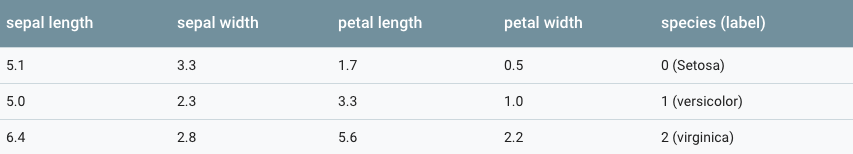
\includegraphics[\textwidth]{images/table}
  \caption{Data representation used for modeling (taken from~\cite{tensor18})}
  \label{fig: rep}
\end{figure}

Although TensorFlow Linear Classifier Estimator was also applicable for this problem, it was required to use the DNNClassifier to perform multi-class classification~\cite{tensor18}. Because the information volume was not very large it was appropriate to develop a four layer model. The two outer layers correspond to the indispensable input and output layers, thus it remains two hidden layers in the net. Continuing with the model development, as implemented in the project above, the first steps to achieve a good model is creating the input functions, and defining the model's feature columns. 

\begin{tensorflow}[caption={ads}]
#Input function definition
def input_evaluation_set():
    features = {'SepalLength': np.array([6.7, 5.3, 4.4]),
                'SepalWidth':  np.array([3.4., 4.2, 3.1]),
                'PetalLength': np.array([5.6, 3.3, 4.8]),
                'PetalWidth':  np.array([2.2, 1.0, 2.8])}
    labels = np.array([3, 1])
    return features, labels
\end{tensorflow}

Interestingly the results obtained by the model classification should sum up to one. In other words, the model was designed to respond to each input by deciding in which proportion the data corresponds to one of the three available flowers. 

\begin{enumerate}
 \item 0.08 for Iris Setosa
 \item 0.02 for Iris Versicolor
 \item 0.90 for Iris Virginica
\end{enumerate}

From the above example it is possible to conclude that the model determined that there was a 90 percent probability that the data corresponded to an Iris Virginica. 
Specifically entering into details concerning the Neural Network development, the DNNClassifier mentioned above provided accesible tools to create the net.

\begin{tensorflow}[caption={ads}]
# Net contains 2 hidden layers with 10 nodes each.
classifier = tf.estimator.DNNClassifier(
    feature_columns=my_feature_columns,
    hidden_units=[10, 10],
# The model must choose between 3 classes which represent each flower.
    n_classes=3)
\end{tensorflow}
Following this, the concluding process was developed in a similar manner to the first project. Namely, training the model and evaluating proceeded. Just like in the first  application, training was implemented using the Estimators train method. 

%%%%
\subsection{Experiments Analysis}
\authorcomment[missing]{}{Why is better to to linear regression than neural networks for supervised learning applications, and viceversa}

For both the Housing and Flower problems models were trained and predictions were made.  From here evaluations were made concluding that indeed linear regression models present useful solutions while keeping things simple. 

The second project developed with data and guidance provided by TensorFlow where the main goal was to classify flowers based on a dataset containing plant measurements such as sepal length, sepal width, petal length and petal width. The Model had to classify the data into one of three iris flowers: Iris setosa, Iris versicolor and Iris virginica.  As said before in this document, it was necessary to set a representation of these classifications for the model to work. Contrary to the method implemented in the first project (supervised machine learning with linear regression) to solve this problem a Deep Neural Network model was implemented. 


%%%%
\subsection{Threads to Validity}



\endinput



